% ============================================================================
% Deep Surrogates to Estimate Dynamic Models
% Summer School on AI for Economics and Finance
% University of Padova, 23-24 September 2026
% Duration: 55 minutes
% ============================================================================

\documentclass[aspectratio=169,11pt]{beamer}

% ---------- Theme and colors ----------
\usecolortheme{dove}
\setbeamertemplate{navigation symbols}{}
\setbeamertemplate{footline}{%
  \hfill\usebeamerfont{page number in head/foot}%
  \usebeamercolor[fg]{normal text}%
  \insertframenumber\,/\,\inserttotalframenumber\kern1em\vskip4pt}
\setbeamerfont{frametitle}{size=\huge}

% ---------- Packages ----------
\usepackage[utf8]{inputenc}
\usepackage[T1]{fontenc}
\usepackage{amsmath,amssymb,amsfonts}
\usepackage{bm}
\usepackage{graphicx}
\usepackage{tikz}
\usetikzlibrary{shapes,arrows.meta,positioning,calc,fit,backgrounds,patterns,decorations.pathreplacing}
\usepackage{pgfplots}
\pgfplotsset{compat=1.18}
% --- readable-from-the-back defaults for every plot ---
\pgfplotsset{every axis/.append style={
    tick label style={font=\footnotesize},
    label style={font=\small},
    title style={font=\small},
    legend style={font=\footnotesize}}}
\usepgfplotslibrary{fillbetween}
\usepackage{booktabs}
\usepackage{hyperref}
\usepackage{multicol}
\usepackage{xcolor}
\usepackage{algorithmic}
\usepackage{listings}
\usepackage{pifont}
\usepackage{array}
\newcommand{\yes}{\textcolor{darkgreen}{\ding{51}}}
\newcommand{\no}{\textcolor{harvardcrimson}{\ding{55}}}
\newcommand{\mixed}{\textcolor{softorange}{\ding{108}}}

% ---------- Tighter display math, applied uniformly at every font size ------
% (a global typographic setting, so that no frame needs a local \vspace hack)
\makeatletter
\g@addto@macro\normalsize{%
  \setlength\abovedisplayskip{5pt plus 2pt minus 2pt}%
  \setlength\belowdisplayskip{5pt plus 2pt minus 2pt}%
  \setlength\abovedisplayshortskip{2pt plus 1pt}%
  \setlength\belowdisplayshortskip{3pt plus 1pt}}
\g@addto@macro\small{%
  \setlength\abovedisplayskip{4pt plus 2pt minus 2pt}%
  \setlength\belowdisplayskip{4pt plus 2pt minus 2pt}%
  \setlength\abovedisplayshortskip{2pt plus 1pt}%
  \setlength\belowdisplayshortskip{2pt plus 1pt}}
\g@addto@macro\footnotesize{%
  \setlength\abovedisplayskip{3pt plus 2pt minus 2pt}%
  \setlength\belowdisplayskip{3pt plus 2pt minus 2pt}%
  \setlength\abovedisplayshortskip{1pt plus 1pt}%
  \setlength\belowdisplayshortskip{2pt plus 1pt}}
\makeatother

% ---------- Custom colors ----------
\definecolor{uzhblue}{rgb}{0,0,0.5}
\definecolor{uzhgreylight}{RGB}{236,238,241}
\definecolor{uzhgreydark}{RGB}{81,86,94}
\definecolor{harvardcrimson}{RGB}{153,0,0}
\definecolor{unil@blue}{RGB}{0,140,204}
\definecolor{unil@black}{RGB}{35,31,32}
\definecolor{darkgreen}{RGB}{0,100,0}
\definecolor{darkred}{RGB}{139,0,0}
\definecolor{softblue}{RGB}{70,130,180}
\definecolor{softorange}{RGB}{230,159,0}
\definecolor{softgreen}{RGB}{0,158,115}

% ---------- Listings (after the colors it references) ----------
\lstset{
  language=Python,
  basicstyle=\small\ttfamily,
  keywordstyle=\color{uzhblue}\bfseries,
  commentstyle=\color{uzhgreydark}\itshape,
  stringstyle=\color{darkgreen},
  showstringspaces=false,
  breaklines=true,
  frame=none,
  aboveskip=2pt, belowskip=2pt}

% ---------- Set beamer colors ----------
\setbeamercolor{frametitle}{bg=uzhgreylight, fg=uzhblue}
\setbeamercolor{title}{fg=uzhblue}
\setbeamercolor{structure}{fg=uzhblue}
\setbeamercolor{block title}{bg=unil@blue, fg=white}
\setbeamercolor{block body}{bg=uzhgreylight}
\setbeamercolor{block title alerted}{bg=darkred,fg=white}
\setbeamercolor{block body alerted}{bg=red!5}
\setbeamercolor{block title example}{bg=darkgreen,fg=white}
\setbeamercolor{block body example}{bg=green!5}
\setbeamercolor{item}{fg=unil@black}
\setbeamercolor{normal text}{fg=unil@black}

% ---------- Emphasis and hyperlinks ----------
\newcommand{\emphc}[1]{\textcolor{harvardcrimson}{#1}}
\hypersetup{colorlinks,linkcolor=harvardcrimson,urlcolor=harvardcrimson}

% ---------- Finger-exercise badge ----------
\newcommand{\exercisepause}{%
  \tikz[baseline=(XB.base)]{%
    \node[rectangle, rounded corners=2pt, fill=softgreen!25, draw=softgreen!70!black,
          inner xsep=4pt, inner ysep=1.5pt,
          font=\footnotesize\bfseries, text=darkgreen] (XB) {PAUSE: 5 min};}}

% ---------- Math commands ----------
% One symbol, one meaning. See the notation frame in Part I.
% NOTE: this lecture is an estimation/policy lecture, so theta is the STRUCTURAL
% parameter vector, not the network weights (which the morning deck called theta).
\newcommand{\x}{\bm{x}}
\newcommand{\R}{\mathbb{R}}
\newcommand{\E}[1]{\mathbb{E}\!\left[#1\right]}
\newcommand{\str}{\bm{\theta}}          % structural parameters
\newcommand{\pol}{\bm{\vartheta}}       % policy parameters
\newcommand{\netw}{\bm{w}}              % network weights
\newcommand{\surr}{\phi}                % the surrogate
\DeclareMathOperator*{\argmin}{arg\,min}
\DeclareMathOperator*{\argmax}{arg\,max}

% ---------- Title ----------
\title[SMM -- Padova 2026]%
{Deep Learning for Solving Dynamic Models}
\subtitle{Session 7: Structural estimation via simulated method of moments}
\author{Simon Scheidegger}
\institute[HEC Lausanne]{HEC, University of Lausanne\\[4pt]
{\footnotesize Based on Chen, Didisheim \& Scheidegger (2026), \emph{Journal of Financial Economics} 177, 104222}}
\date{University of Padova\\September 24, 2026}

\begin{document}

% ============================================================================
% PART 0: TITLE & OUTLINE
% ============================================================================

{\setbeamercolor{background canvas}{bg=uzhgreylight}
\begin{frame}
\titlepage
\end{frame}
}

\begin{frame}{Day 2 at a Glance}
\begin{center}
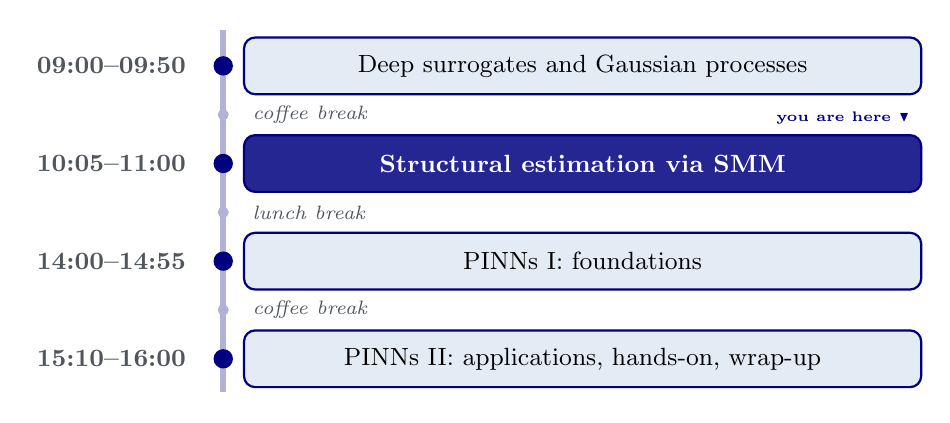
\begin{tikzpicture}[
    session/.style={rectangle, rounded corners=4pt, draw=uzhblue, thick, fill=softblue!15,
                    minimum width=8.6cm, minimum height=0.72cm, align=left, font=\small,
                    inner xsep=10pt, anchor=west},
    now/.style={session, fill=uzhblue!85, draw=uzhblue, text=white, font=\small\bfseries},
    pause/.style={font=\scriptsize\itshape, text=uzhgreydark, anchor=west},
    time/.style={font=\small\bfseries, text=uzhgreydark, anchor=east}
]
    \draw[uzhblue!30, line width=2pt] (0,0.45) -- (0,-4.14);
    \node[time] at (-0.35,0.00) {09:00--09:50};
    \node[session] at (0.25,0.00) {Deep surrogates and Gaussian processes};
    \fill[uzhblue] (0,0.00) circle (3.5pt);
    \node[pause] at (0.25,-0.62) {coffee break};
    \fill[uzhblue!30] (0,-0.62) circle (2pt);
    \node[time] at (-0.35,-1.24) {10:05--11:00};
    \node[now] at (0.25,-1.24) {Structural estimation via SMM};
    \fill[uzhblue] (0,-1.24) circle (3.5pt);
    \node[font=\tiny\bfseries, text=uzhblue, anchor=south east] at (8.85,-0.86) {you are here $\blacktriangledown$};
    \node[pause] at (0.25,-1.86) {lunch break};
    \fill[uzhblue!30] (0,-1.86) circle (2pt);
    \node[time] at (-0.35,-2.48) {14:00--14:55};
    \node[session] at (0.25,-2.48) {PINNs I: foundations};
    \fill[uzhblue] (0,-2.48) circle (3.5pt);
    \node[pause] at (0.25,-3.10) {coffee break};
    \fill[uzhblue!30] (0,-3.10) circle (2pt);
    \node[time] at (-0.35,-3.72) {15:10--16:00};
    \node[session] at (0.25,-3.72) {PINNs II: applications, hands-on, wrap-up};
    \fill[uzhblue] (0,-3.72) circle (3.5pt);
\end{tikzpicture}
\end{center}
\end{frame}

\begin{frame}{Roadmap of This Lecture (55 min)}
\footnotesize
\begin{columns}[T]
\column{0.48\textwidth}
\textbf{I.\ The idea}~~\mbox{\small (12 min)}
\begin{itemize}\setlength\itemsep{1pt}
    \item The estimation loop, and why it is expensive
    \item SMM on one frame; common random numbers
    \item The model and the moments
\end{itemize}

\vspace{0.4em}
\textbf{II.\ One parameter}~~\mbox{\small (18 min)}
\begin{itemize}\setlength\itemsep{1pt}
    \item A policy network with $\varrho$ as an input
    \item Its accuracy against the reference solution
    \item Moments, criterion, estimate (\texttt{07\_01})
    \item The other route: a GP of the moment map
\end{itemize}

\column{0.48\textwidth}
\textbf{III.\ Two parameters}~~\mbox{\small (15 min)}
\begin{itemize}\setlength\itemsep{1pt}
    \item $(\beta, \varrho)$ jointly (\texttt{07\_02})
    \item How sharply each moment set pins down $\beta$
    \item The moment Jacobian in one number
    \item The GP route with two parameters
\end{itemize}

\vspace{0.4em}
\textbf{Finger exercise, production, hands-on}~~\mbox{\small (10 min)}
\end{columns}

\vspace{0.1em}
\begin{center}
{\scriptsize Notebooks in \texttt{day2/code/07\_structural\_estimation/}: \texttt{07\_01\_SMM\_One\_Parameter.ipynb}, \texttt{07\_02\_SMM\_Two\_Parameters.ipynb}}
\end{center}
\end{frame}

\begin{frame}{Learning Objectives}
\textbf{By the end of this lecture you should be able to:}
\begin{itemize}\itemsep4pt
  \item Write down the simulated-method-of-moments criterion and say why every evaluation of it used to require solving the model
  \item Train a policy network with structural parameters as inputs, and validate it against a reference solution across the parameter range
  \item Simulate moments under common random numbers and minimize the criterion on the fly, for one parameter and for two, and do the same with Gaussian processes of the moment map fit to a handful of solves
  \item Read a criterion surface: say how sharply a moment set pins down each parameter, and confirm it with the moment Jacobian
\end{itemize}
\end{frame}

% ============================================================================
% PART I: THE IDEA
% ============================================================================

\begin{frame}{}
\begin{center}
{\Huge \textcolor{uzhblue}{Part I}}\\[0.8em]
{\LARGE The Idea}
\end{center}
\end{frame}

% --- The estimation loop ---
\begin{frame}{The Estimation Loop, and Why It Is Expensive}
\small
\textbf{The nested loop.} For each candidate $\str$:
\begin{center}
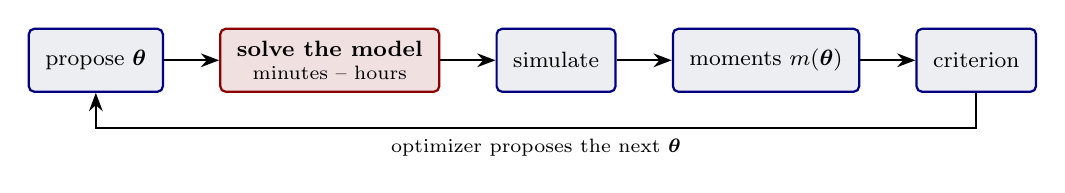
\begin{tikzpicture}[
    box/.style={rectangle, draw=uzhblue, thick, rounded corners=2pt, fill=uzhgreylight,
                minimum height=0.8cm, font=\footnotesize, align=center, inner xsep=6pt},
    >=Stealth
]
\node[box] (guess) {propose $\str$};
\node[box, right=0.7cm of guess, fill=darkred!12, draw=darkred] (solve) {\textbf{solve the model}\\[-1pt]{\scriptsize minutes -- hours}};
\node[box, right=0.7cm of solve] (sim) {simulate};
\node[box, right=0.7cm of sim] (mom) {moments $m(\str)$};
\node[box, right=0.7cm of mom] (crit) {criterion};
\draw[->, thick] (guess) -- (solve);
\draw[->, thick] (solve) -- (sim);
\draw[->, thick] (sim) -- (mom);
\draw[->, thick] (mom) -- (crit);
\draw[->, thick] (crit.south) -- ++(0,-0.45) -| node[pos=0.25, below, font=\scriptsize] {optimizer proposes the next $\str$} (guess.south);
\end{tikzpicture}
\end{center}

\vspace{0.25cm}
\textbf{The surrogate move.} Train the policy network with $\str$ as an input, once. The red box is then gone from the loop: a candidate $\str$ costs one simulation of the network, and the loop runs on the fly.

\vspace{0.15cm}
\begin{block}{Two consequences}
The criterion is cheap enough to evaluate on a grid, so you can \emph{look at} it rather than trust a local optimizer's report; and under common random numbers it is smooth in $\str$, so a standard minimizer finishes the job.
\end{block}
\end{frame}


\begin{frame}{SMM on One Frame}
\footnotesize
\textbf{Data:} $T$ observations $\{y_t\}$, summarized by $q$ moments $\hat m = \frac1T \sum_t g(y_t)$: here standard deviations, autocorrelations, a mean.

\textbf{Model:} for a candidate $\str$, simulate a sample of length $S$ and compute the same moments, $m(\str)$.

\begin{block}{The estimator}
\vspace{-4pt}
\[
\hat\str = \argmin_{\str}\; Q(\str), \qquad Q(\str) = \big[m(\str) - \hat m\big]^\top W \big[m(\str) - \hat m\big], \qquad W = I \text{ here.}
\]
\vspace{-8pt}
\end{block}

\begin{itemize}\itemsep1pt
  \item $q \ge p$ moments for $p$ parameters; with $q > p$ the criterion cannot reach zero and its minimum is a compromise across moments.
  \item $W = I$ is consistent and simple; the efficient choice, the inverse covariance of the data moments, changes the standard errors, not the picture.
  \item \emphc{Identification}: $\str_0$ is the unique minimizer of the population criterion, so the moments must \emph{move} with every parameter (Part III).
\end{itemize}

\vspace{-0.05cm}
\begin{alertblock}{Common random numbers}
Use the \emphc{same} shock sequence for every candidate $\str$. Then $m(\str)$ is a smooth function and $Q$ has a clean minimum. Redraw the shocks and the minimizer chases simulation noise.
\end{alertblock}
\end{frame}

\begin{frame}{The Model: Brock--Mirman with Stochastic TFP}
\footnotesize
\vspace{-0.3cm}
The economy of Session 2, with $\delta = 0.10$ so that no closed form exists and the Euler equation has to be solved:
\begin{gather*}
\max_{\{C_t\}} \sum_{t=0}^{\infty} \beta^t\, \E{\ln C_t},
\qquad K_{t+1} + C_t = Y_t + (1-\delta)K_t ,\\[4pt]
Y_t = z_t K_t^{\alpha}, \qquad
\log z_{t+1} = \varrho \log z_t + \sigma\,\varepsilon_{t+1},
\qquad \varepsilon_{t+1} \sim \mathcal{N}(0,1).
\end{gather*}

\vspace{0.1cm}
\begin{columns}[T]
\column{0.40\textwidth}
\textbf{Calibration}
\begin{center}\footnotesize
\begin{tabular}{cccc}
\toprule
$\alpha$ & $\delta$ & $\sigma$ & $\beta$ (Part II) \\
\midrule
$0.36$ & $0.10$ & $0.04$ & $0.96$ \\
\bottomrule
\end{tabular}
\end{center}
\vspace{0.1cm}
\textbf{Truth for the synthetic data:} $\varrho = 0.90$, and in Part III $\beta = 0.96$.

\column{0.58\textwidth}
\textbf{Four moments, and which parameter each responds to}
\begin{center}\footnotesize
\setlength{\tabcolsep}{4pt}
\begin{tabular}{lll}
\toprule
moment & in $\varrho$ & in $\beta$ \\
\midrule
$\mathrm{Std}(\Delta \log C_t)$ & rises above $0.8$ & weak \\
$\mathrm{Corr}(\Delta \log C_t, \Delta \log C_{t-1})$ & rises to $0.9$, falls after & weak \\
$\mathrm{Corr}(\log Y_t, \log Y_{t-1})$ & rises throughout & none \\
$\mathrm{mean}(I_t / Y_t)$ & none & rises \\
\bottomrule
\end{tabular}
\end{center}
{\scriptsize $\varrho$ sets how long shocks last, so the autocorrelations respond to it. $\beta$ sets the steady-state capital stock, $k^\star = \big(\alpha / (1/\beta - 1 + \delta)\big)^{1/(1-\alpha)}$, so only a level moment responds to it. Measured in \texttt{07\_01} and \texttt{07\_02}.}
\end{columns}
\end{frame}

\begin{frame}{The Reference Solution, and the Data}
\small
\textbf{Reference solver} (\texttt{brock\_mirman\_reference.py}): iterate on the Euler equation with cash on hand as the state (endogenous grid method, cubic splines) until the consumption function stops changing. Relative Euler errors below $10^{-6}$ on the ergodic set at every corner of the parameter box; about 1.7 s per solve.

\vspace{0.2cm}
\textbf{The data:} one path of $T = 500$ periods from the reference solution at the true parameters, with its own shocks. Its four moments are the targets $\hat m$.

\vspace{0.2cm}
\begin{block}{What the reference solver is for}
Not for the estimation, where it would be the expensive red box. For \emphc{validating the surrogate}, at several parameter values, on the states the model visits; and, once, for drawing the criterion the true model would give, so that the surrogate's criterion can be laid on top of it.
\end{block}
\end{frame}

% ============================================================================
% PART II: ONE PARAMETER
% ============================================================================

\begin{frame}{}
\begin{center}
{\Huge \textcolor{uzhblue}{Part II}}\\[0.8em]
{\LARGE One Parameter: $\varrho$}
\end{center}
\end{frame}

\begin{frame}{Step 1: A Policy Network with $\varrho$ as an Input}
\small
\begin{block}{The surrogate}
$(\log z_t, K_t, \varrho) \mapsto$ consumption share of cash on hand $m_t = Y_t + (1-\delta)K_t$, through a sigmoid, so $0 < C_t < m_t$ by construction and $K_{t+1} = m_t - C_t$.
\end{block}

\vspace{0.1cm}
\textbf{Loss:} the relative Euler residual, with five Gauss--Hermite nodes for the expectation,
\[
e(z, K, \varrho) = 1 - \frac{1}{\beta\, C_t\, \mathbb{E}_t\!\left[\dfrac{1 - \delta + \alpha z_{t+1} K_{t+1}^{\alpha-1}}{C_{t+1}}\right]},
\qquad \mathcal{L} = \frac1N \sum_i e_i^2 .
\]
\textbf{States:} each batch is half uniform draws over a box in $(\log z, K, \varrho)$, half states visited by simulating the current policy, so the network is accurate where the estimator will evaluate it.

\vspace{0.2cm}
\emphc{Nothing about $\varrho$ is special.} It enters the transition $\log z_{t+1} = \varrho \log z_t + \sigma\varepsilon$ inside the expectation, and the Euler residual is zero for every value of it. One training run, 2 min, covers $\varrho \in [0.50, 0.99]$.
\end{frame}

\begin{frame}{Step 1, Checked Against the Reference Solution}
\begin{center}
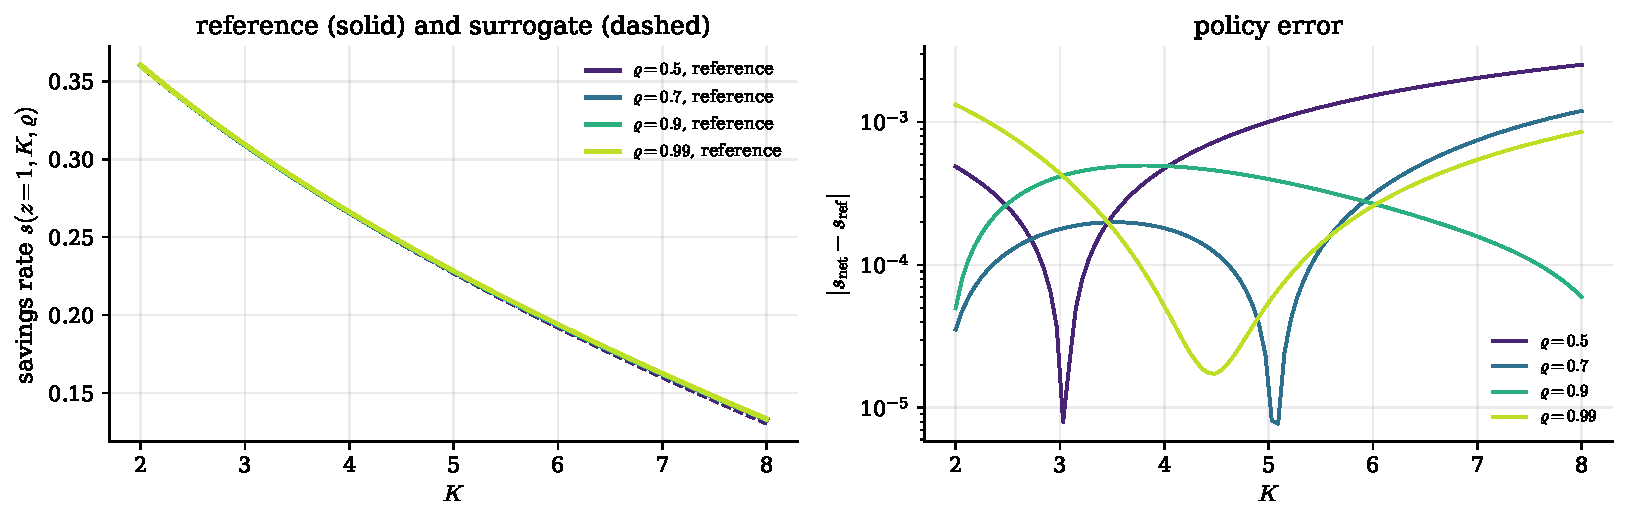
\includegraphics[width=0.84\linewidth]{figures/smm1_surrogate_accuracy.pdf}
\end{center}
\vspace{-0.25cm}
{\scriptsize Notebook \texttt{07\_01}, stored teaching run. On 2{,}000 ergodic states per $\varrho$: $\varrho=0.5$: mean Euler error $1.6\cdot10^{-4}$, mean consumption error $8.3\cdot10^{-4}$, max $1.3\cdot10^{-3}$; $\varrho=0.7$: mean Euler error $5.5\cdot10^{-5}$, mean consumption error $2.1\cdot10^{-4}$, max $4.9\cdot10^{-4}$; $\varrho=0.9$: mean Euler error $1.1\cdot10^{-4}$, mean consumption error $5.7\cdot10^{-4}$, max $7.1\cdot10^{-4}$; $\varrho=0.99$: mean Euler error $2.5\cdot10^{-4}$, mean consumption error $1.1\cdot10^{-3}$, max $2.1\cdot10^{-2}$.. The consumption error is the number that matters for estimation; the Euler residual is only the training loss.}
\end{frame}

\begin{frame}{Step 2: $\varrho$ Moves the Simulated Moments}
\begin{center}
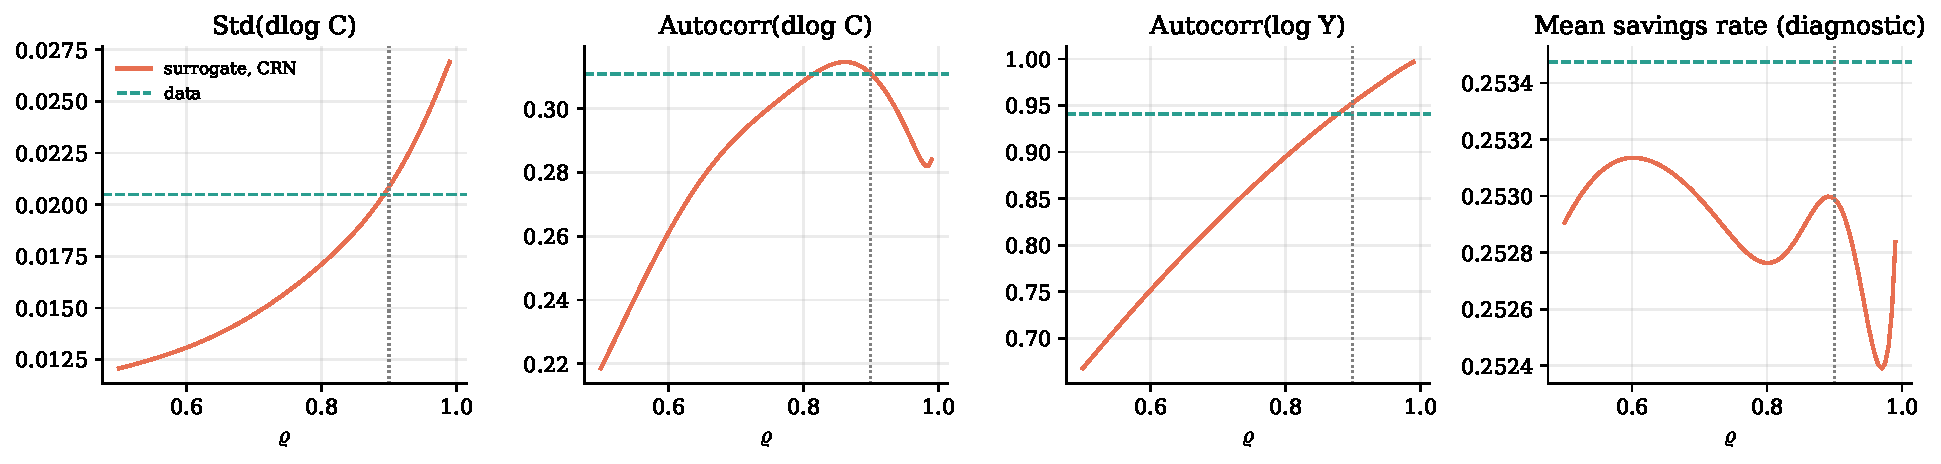
\includegraphics[width=0.98\linewidth]{figures/smm1_moments.pdf}
\end{center}
\vspace{-0.1cm}
{\small 99 candidates from $0.50$ to $0.99$, each simulated for 2,000 periods from the same state under the \emphc{same} shocks, in 1 s. Every moment used moves with $\varrho$, so the data moments (dashed) pin it down; the mean investment share does not move with $\varrho$ and is left out. Notebook \texttt{07\_01}, stored teaching run.}
\end{frame}

\begin{frame}{Step 3: The Criterion and the Estimate}
\begin{center}
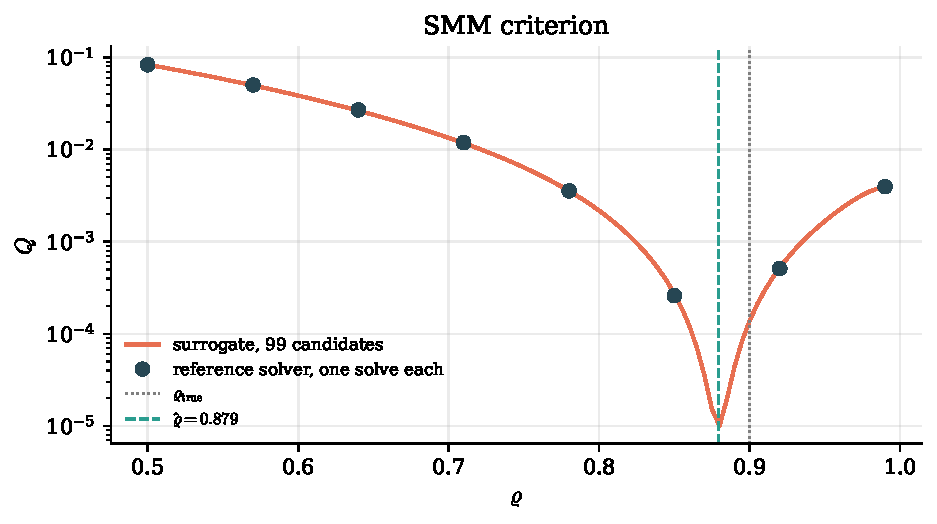
\includegraphics[width=0.52\linewidth]{figures/smm1_criterion.pdf}
\end{center}
\vspace{-0.2cm}
{\footnotesize Notebook \texttt{07\_01}. The surrogate's criterion on 99 candidates, and the reference solver's on 8 candidates, one solve each. Grid minimum, then a bounded scalar minimizer: $\hat\varrho = $ 0.8793. \textbf{The surrogate's curve lies on the reference solver's points}: the surrogate adds no visible error. \textbf{The minimum is at 0.8793, not $0.90$, for both}: that is the sampling error of a 500-period sample (its output autocorrelation is 0.941 against a population value of 0.947; across 200 such samples the sampling standard deviation is 0.0127).}
\end{frame}

\begin{frame}{The Other Route: a GP of the Moment Map}
\begin{center}
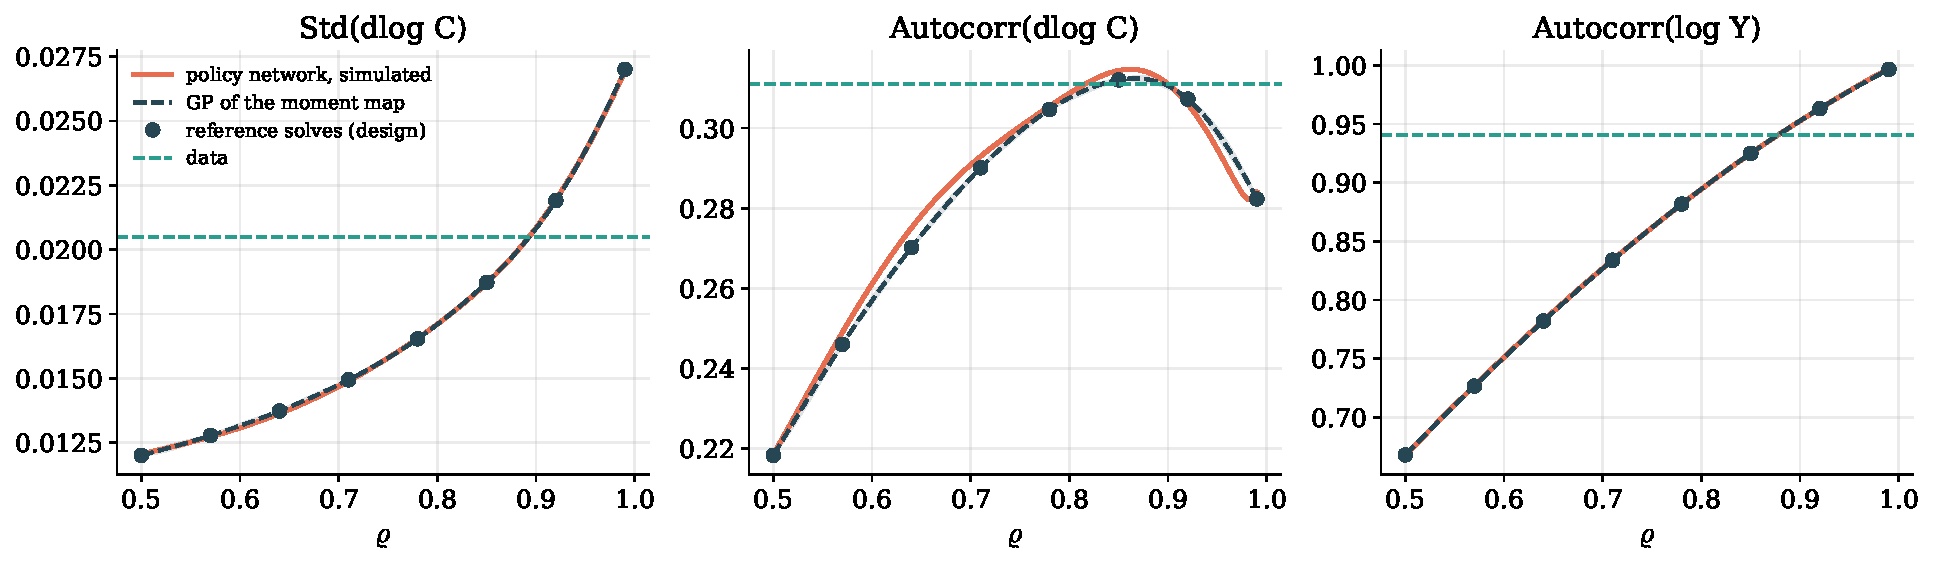
\includegraphics[width=0.9\linewidth]{figures/smm1_gp_route.pdf}
\end{center}
\vspace{-0.2cm}
{\small The network is a surrogate of the \emph{policy}, simulated at every candidate. The other kind of surrogate from Session 6 fits the \emph{moment map} $m_j(\varrho)$ directly: one GP per moment on 8 reference solves (dots), Matérn 5/2, hyperparameters by marginal likelihood. Its posterior mean replaces the simulation in $Q$; the band is its own error bar. Estimate: 0.8784 by the GP route against 0.8793 by the network route, truth $0.90$. Notebook \texttt{07\_01}, Section 6.}
\end{frame}

% ============================================================================
% PART III: TWO PARAMETERS
% ============================================================================

\begin{frame}{}
\begin{center}
{\Huge \textcolor{uzhblue}{Part III}}\\[0.8em]
{\LARGE Two Parameters: $(\beta, \varrho)$}
\end{center}
\end{frame}

\begin{frame}{The Same Surrogate, One More Input}
\small
$(\log z_t, K_t, \beta, \varrho) \mapsto$ consumption share; the Euler residual with $\beta$ read from the input. Box $\beta \in [0.92, 0.99]$, $\varrho \in [0.50, 0.99]$; the capital box is wide enough for every $\beta$'s ergodic set.

\vspace{0.15cm}
\textbf{Checked at five corners and the centre of the box}, on 2{,}000 ergodic states each:
\begin{center}
\footnotesize
\begin{tabular}{cc cc cc}\toprule $\beta$ & $\varrho$ & mean Euler & max Euler & mean $|\Delta C|/C$ & max $|\Delta C|/C$ \\ \midrule 0.92 & 0.5 & $1.3\cdot10^{-4}$ & $3.5\cdot10^{-4}$ & $4.2\cdot10^{-4}$ & $7.6\cdot10^{-4}$ \\ 0.92 & 0.99 & $1.8\cdot10^{-4}$ & $1.1\cdot10^{-3}$ & $5.9\cdot10^{-4}$ & $3.0\cdot10^{-3}$ \\ 0.96 & 0.9 & $3.1\cdot10^{-5}$ & $1.9\cdot10^{-4}$ & $9.8\cdot10^{-5}$ & $5.3\cdot10^{-4}$ \\ 0.99 & 0.5 & $3.0\cdot10^{-4}$ & $4.4\cdot10^{-4}$ & $2.3\cdot10^{-3}$ & $2.9\cdot10^{-3}$ \\ 0.99 & 0.99 & $5.3\cdot10^{-4}$ & $5.1\cdot10^{-3}$ & $3.7\cdot10^{-3}$ & $3.3\cdot10^{-2}$ \\ \bottomrule\end{tabular}
\end{center}

\vspace{0.1cm}
\begin{alertblock}{Why the check comes first}
A criterion that is flat in $\beta$ has two possible causes: the moments do not respond to $\beta$, or the \emph{surrogate} does not. Only the comparison with the reference solution tells them apart. The table rules the second out here.
\end{alertblock}
\end{frame}

\begin{frame}{How Sharply Each Moment Set Pins Down $\beta$}
\vspace{-0.25cm}
\begin{columns}[T]
\column{0.66\textwidth}
\begin{center}
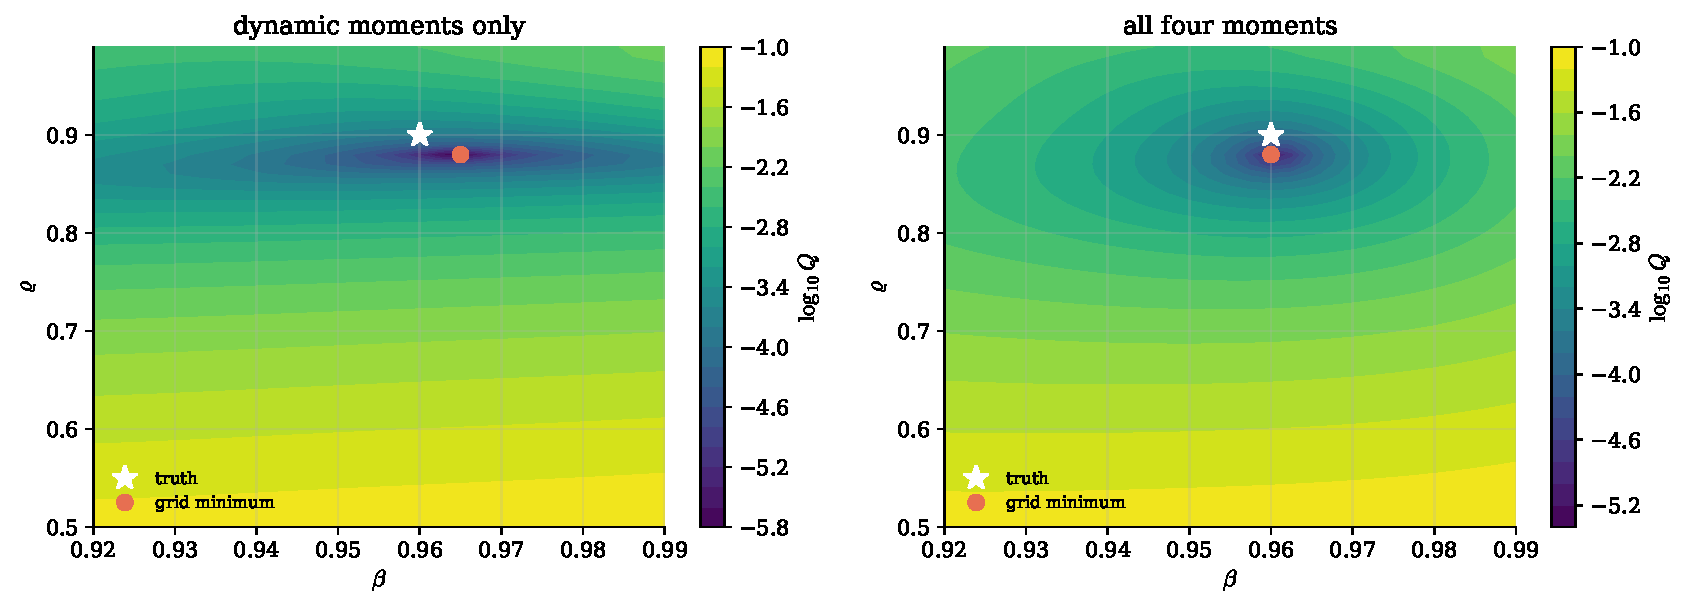
\includegraphics[width=\linewidth]{figures/smm2_criterion_surfaces.pdf}
\end{center}
\column{0.32\textwidth}
\vspace{0.3cm}
\footnotesize
\textbf{Floor of each surface}, $\min_\varrho Q(\beta, \varrho)$:
\begin{center}
\renewcommand{\arraystretch}{1.05}
\setlength{\tabcolsep}{4pt}
{\scriptsize
\begin{tabular}{lrr}
\toprule
$\beta$ & dynamic only & all four \\
\midrule
0.920 & $3.4\cdot10^{-4}$ & $4.2\cdot10^{-3}$ \\
0.960 & $5.6\cdot10^{-6}$ & $6.2\cdot10^{-6}$ \\
0.990 & $1.4\cdot10^{-4}$ & $5.3\cdot10^{-3}$ \\
\bottomrule
\end{tabular}}
\end{center}
\end{columns}
\vspace{-0.2cm}
{\footnotesize 1,450 candidates under common random numbers, $\log_{10} Q$; left the three dynamic moments, right with the mean investment share added. Both find the same minimum. Moving $\beta$ from $0.96$ to the edge of the box raises the criterion by a factor 25 to 60 with the dynamic moments, by 700 to 850 with the level moment added: \textbf{the dynamic moments identify $\beta$, but 12 to 37 times more weakly}, so a small error in the moments moves $\hat\beta$ far along the left surface and little along the right one. \emphc{Identification is fixed by information, not by a better optimizer.} Notebook \texttt{07\_02}.}
\end{frame}

\begin{frame}{The Moment Jacobian in One Number}
\footnotesize
At the estimate, by central differences on the surrogate, with the parameters scaled to the box, $u = (\str - \str_{\rm lo})/(\str_{\rm hi} - \str_{\rm lo})$, so that a step of one is a step across the plotted range in either direction (in raw units the $\beta$ column would be seven times smaller only because the box is seven times narrower):
\[
M = \frac{\partial m}{\partial u} \in \R^{q \times 2}, \qquad M = U\,\mathrm{diag}(s_1, s_2)\,V^\top .
\]
Near the minimum $Q \approx \delta u^\top M^\top M\, \delta u$, so $s_2^2$ is the criterion's curvature in its flattest direction and the last column of $V$ names that direction. This is the previous frame in one number.

\vspace{0.1cm}
\begin{center}
\renewcommand{\arraystretch}{1.05}
\begin{tabular}{lccc}
\toprule
moments & $s_1$ & $s_2$ & flattest direction $(\beta, \varrho)$ \\
\midrule
dynamic only & 0.273 & 0.0320 & $(-1.00, -0.01)$ \\
all four & 0.272 & 0.1419 & $(-1.00, -0.02)$ \\
\bottomrule
\end{tabular}
\end{center}

\vspace{0.1cm}
Estimates: dynamic moments only $(\hat\beta, \hat\varrho) = (0.9641, 0.8786)$; all four moments $(0.9605, 0.8782)$; truth $(0.96, 0.90)$. The ratio of singular values falls from 9 to 2 when the level moment is added.

\vspace{0.05cm}
{\scriptsize With an efficient $W$ and the covariance of the data moments, $(M^\top W M)^{-1}$ scaled by $1/T$ is the asymptotic variance of $\hat u$; a small $s_2$ is a large standard error along $V_{\cdot 2}$. The notebooks stop at $M$; the covariance is one more simulation away.}
\end{frame}

\begin{frame}{The GP Route With Two Parameters}
\begin{center}
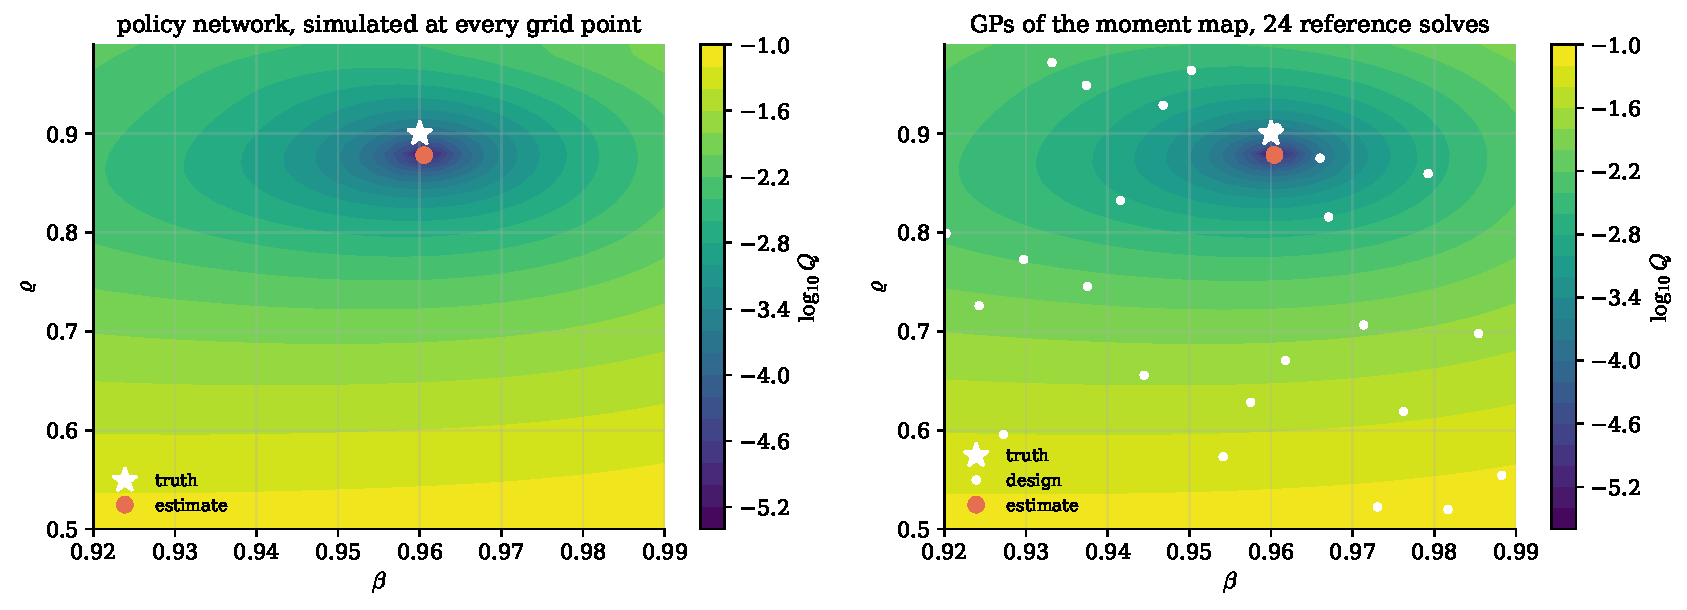
\includegraphics[width=0.82\linewidth]{figures/smm2_gp_route.pdf}
\end{center}
\vspace{-0.2cm}
{\small Left: the criterion from the policy network, simulated at every grid point. Right: the criterion from four GPs of the moment map fit to 24 reference solves on a Latin-hypercube design (dots). Estimates $(0.9604, 0.8785)$ by the GP route, $(0.9605, 0.8782)$ by the network route, truth $(0.96, 0.90)$. The two routes agree; what differs is the cost curve: the network adds one input per parameter and trains once, the GP needs a design that fills one more dimension per parameter and carries an error bar for it. Notebook \texttt{07\_02}, Section 6.}
\end{frame}

\begin{frame}{The Surrogate Is Not Free}
\small
The moments came from the network, not from the model: $m_{\rm net}(\str) = m(\str) + e(\str)$.

\begin{alertblock}{$e$ does not shrink with the sample}
More data makes $\hat m$ precise; it does nothing to $e$. The estimator converges to the minimizer of the criterion built on $m_{\rm net}$, which is the truth only to the extent that $e$ is small \emph{across the parameter range}.
\end{alertblock}

\vspace{0.2cm}
\textbf{The practical rule.} Report the surrogate's \emphc{maximum} consumption error over the parameter box against a reference solution, on the states the model visits, before reporting an estimate. In \texttt{07\_01} that maximum is $2.1\cdot10^{-2}$; in \texttt{07\_02} it is $3.3\cdot10^{-2}$. If it is not small relative to how much the moments move, train longer or widen the state box, and check again.

\vspace{0.2cm}
{\footnotesize Chen, Didisheim \& Scheidegger (2026), fn.\ 15, make the same point about their own surrogate.}
\end{frame}

\begin{frame}{Finger Exercise: Which Moment Moves With $\varrho$?}
\begin{flushright}\exercisepause{}\end{flushright}
\vspace{-0.35cm}
\begin{exampleblock}{The setting}
$\log z_{t+1} = \varrho \log z_t + \sigma \varepsilon_{t+1}$ with $\varepsilon \sim \mathcal N(0,1)$, stationary.
\end{exampleblock}

\vspace{0.3cm}
\begin{enumerate}\itemsep6pt
  \item Compute $\mathrm{Var}(\log z_t)$ and $\mathrm{Var}(\Delta \log z_t)$ as functions of $\varrho$ and $\sigma$.
  \item Which of the two rises with $\varrho$, and which falls?
  \item Output is $Y_t = z_t K_t^\alpha$ and capital moves slowly. Which of the four moments on the model frame should respond most to $\varrho$, and in which direction? Check against the moment figure of Part II.
\end{enumerate}
\end{frame}

\begin{frame}{Solution: Which Moment Moves With $\varrho$?}
\small
\begin{block}{1. The two variances}
Stationarity gives $\mathrm{Var}(\log z) = \sigma^2 / (1 - \varrho^2)$. For the difference, $\Delta \log z_t = (\varrho - 1)\log z_{t-1} + \sigma\varepsilon_t$, so
$\mathrm{Var}(\Delta \log z) = (1-\varrho)^2 \dfrac{\sigma^2}{1-\varrho^2} + \sigma^2 = \dfrac{2\sigma^2}{1 + \varrho}$.
\end{block}

\begin{block}{2. Directions}
The level variance \emphc{rises} without bound as $\varrho \to 1$; the variance of the difference \emphc{falls}, from $2\sigma^2$ at $\varrho = 0$ to $\sigma^2$ at $\varrho = 1$. A more persistent process wanders further but changes less from one period to the next.
\end{block}

\begin{block}{3. The moments}
$\mathrm{Corr}(\log Y_t, \log Y_{t-1})$ inherits the autocorrelation of $\log z$, close to $\varrho$ itself, and rises steeply. $\mathrm{Std}(\Delta \log C)$ follows the falling variance of the difference, dampened by consumption smoothing, so it moves little. The mean investment share depends on the level of capital, which $\varrho$ hardly touches. That is the ordering in the Part II figure.
\end{block}
\end{frame}

\begin{frame}{From Classroom to Production}
\small
Brock--Mirman is the mechanism in miniature. Chen, Didisheim \& Scheidegger (2026) run it on a high-dimensional option-pricing model, with a network in place of a Fourier-transform pricer.

\vspace{0.2cm}
\begin{columns}[T]
\column{0.48\textwidth}
\textbf{What the surrogate enables}
\begin{itemize}\itemsep1pt
  \item Re-estimate \emphc{every day} instead of once per paper
  \item Systematic out-of-sample evaluation against reduced-form benchmarks
  \item Conditional distributions of option returns
\end{itemize}

\column{0.48\textwidth}
\textbf{What that produced}
\begin{itemize}\itemsep1pt
  \item An option-implied \emphc{tail-risk index}, predictive of market crashes
  \item A \emphc{parameter-instability} measure that lines up with option-market illiquidity
  \item A read on the structural-versus-reduced-form trade-off
\end{itemize}
\end{columns}

\vspace{0.25cm}
\begin{alertblock}{The pattern worth remembering}
None of these are faster versions of old results. They are questions whose \emph{answers require a time series of estimates}, and that is what a surrogate with the parameters as inputs manufactures.
\end{alertblock}
\end{frame}

\begin{frame}{Summary, and What to Run}
\footnotesize
\vspace{-0.2cm}
\begin{enumerate}\itemsep1pt
  \item The expensive step in SMM is the model solve inside the loop. A policy network with the parameters as inputs is trained once and removes it.
  \item Validate the surrogate against a reference solution across the parameter range before estimating with it; the Euler residual is not that validation.
  \item Common random numbers make the simulated moments smooth; then a grid shows the criterion and a standard minimizer finishes it.
  \item Identification is a property of the moments. A criterion that is flat along a parameter is either the moments or the surrogate; the reference check tells which, and the moment Jacobian puts a number on it.
  \item Two surrogates, one estimate: a policy network simulated on the fly, or Gaussian processes of the moment map fit to a few solves. Both replace the solve in the loop; the label budget and the number of parameters decide between them.
\end{enumerate}

\vspace{0.1cm}
\begin{block}{Hands-on, \texttt{day2/code/07\_structural\_estimation/}}
\texttt{07\_01\_SMM\_One\_Parameter.ipynb} (3 min) and \texttt{07\_02\_SMM\_Two\_Parameters.ipynb} (8 min), teaching presets stored; set \texttt{RUN\_MODE = "smoke"} in class. Try: change the true $\varrho$; drop a moment; shorten the observed sample to $T = 100$ and watch the criterion's minimum move.
\end{block}
\end{frame}

\begin{frame}{}
\begin{columns}[c]
\column{0.42\textwidth}
\begin{center}
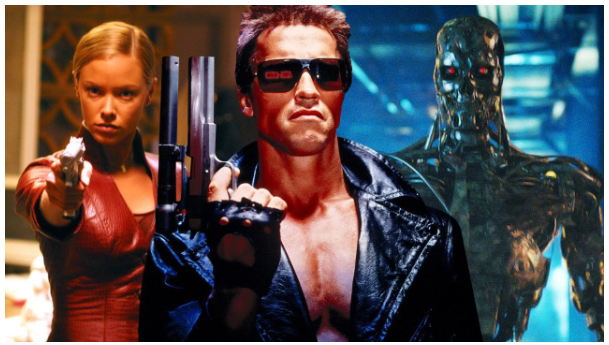
\includegraphics[width=0.8\linewidth]{figures/quest.png}
\end{center}
\column{0.55\textwidth}
{\LARGE \textcolor{uzhblue}{Questions?}}

\vspace{0.5cm}
{\small
\textbf{Simon Scheidegger}\\
HEC, University of Lausanne\\[4pt]
\href{mailto:simon.scheidegger@unil.ch}{simon.scheidegger@unil.ch}~~$\cdot$~~\href{https://sischei.github.io}{sischei.github.io}
}

\vspace{0.5cm}
{\footnotesize
\textbf{Next up, Session 8:} \emph{Economics-informed neural networks: foundations.}
}

\vspace{0.4cm}
{\footnotesize
\textbf{Materials:}\\ \href{https://github.com/sischei/deep_learning_padova_0926}{github.com/sischei/deep\_learning\_padova\_0926}
}
\end{columns}
\end{frame}

\end{document}
